% /Users/pikachu/books/payments-book/src/parts/part4/ch25-alternative-methods.tex
\chapter{Альтернативные методы: QR, BNPL, крипто, цифровой рубль}
\label{ch:alt-methods}
\margintoc

\begin{kaobox}[title=Что вы узнаете из этой главы]
  Карты --- не единственный способ заплатить, хотя в большинстве стран именно
  они задают базовый пользовательский сценарий. Из этой главы вы узнаете,
  как классифицировать методы оплаты по единой системе признаков; как
  устроены QR-платежи в трёх разных моделях --- СБП, Alipay и PIX; как
  работает BNPL на уровне протокола, а не только маркетинга; что такое цифровая
  валюта центрального банка (central bank digital currency, CBDC) и чем она
  архитектурно отличается от безналичных денег; и почему карточные контуры
  сохраняют доминирование несмотря на рост альтернатив.
\end{kaobox}

Чтобы не превратить главу в витрину брендов, будем держать три оси
сравнения: кто авторизует платёж, где происходит расчёт и на ком остаётся
риск спора или невозвратности. Тогда QR, BNPL, CBDC и crypto перестают
быть модными ярлыками и складываются в сравнимые архитектуры.

\section{Таксономия методов оплаты}
\label{sec:alt-taxonomy}

Разговор об альтернативных методах оплаты часто страдает от отсутствия
общего языка: \enquote{кошелёк}, \enquote{перевод}, \enquote{BNPL} ---
слова, за которыми могут стоять принципиально разные архитектуры. Единая
таксономия помогает сравнивать методы по существенным параметрам, а не по
маркетинговым описаниям.

Первый и наиболее распространённый класс --- карточные платежи (card
payments): pull-инструмент, при котором мерчант инициирует списание по
карточным реквизитам клиента. Его сильные стороны --- глобальная
инфраструктура, chargeback и зрелый PCI DSS-контур; его слабая сторона ---
стоимость. В эту группу входят \scheme{Visa}, \scheme{Mastercard},
\scheme{Мир}, UnionPay и AmEx.

Второй класс --- счёт-счёт (account-to-account, A2A): push-инструмент, при
котором клиент сам авторизует перевод со своего счёта на счёт мерчанта.
Примеры --- СБП, SEPA Instant Credit Transfer, UK Faster Payments, PIX
(Бразилия) и UPI (Индия). Сильная сторона A2A --- финальность и низкие
комиссии; слабая --- более узкая защита покупателя.

Третий класс --- кошельки: надстройка над базовым платёжным контуром. Замкнутый кошелёк
(closed-loop wallet) хранит деньги внутри экосистемы, как у Alipay и WeChat
Pay; открытый кошелёк (open-loop wallet) лишь оборачивает карточный
инструмент токеном, как Apple Pay или Google Pay.

Четвёртый класс --- BNPL (Buy Now Pay Later). Здесь я добавляю
\sidenote{BNPL --- buy now, pay later: провайдер оплачивает мерчанту всю
сумму сразу, а клиент возвращает её частями по собственному графику.}
подсказку, потому что термин в книге встречается впервые здесь. Мерчант
получает полную сумму немедленно от BNPL-провайдера, а потребитель
выплачивает её частями. С точки зрения мерчанта это действительно похоже
на эквайринг с другой комиссией, но экономическая модель у такого потока
иная.

Пятый класс --- наличный сценарий (cash-based): платёж начинается онлайн,
а завершается офлайн через ваучер или код. Примеры --- Boleto Bancário в
Бразилии, Oxxo Pay в Мексике, терминалы QIWI. Ключевой параметр здесь ---
задержка подтверждения: деньги приходят не мгновенно.

Шестой класс --- цифровая валюта центрального банка (central bank digital
currency, CBDC): деньги центрального банка в цифровой форме. Это отдельный
реестр, а не банковский депозит.

Наконец, криптовалюты --- децентрализованные токены или стейблкоины.
Их сильная сторона --- программируемость и трансграничность; слабая ---
волатильность, регуляторная неоднородность и нишевое применение.

\begin{figure}
  \centering
  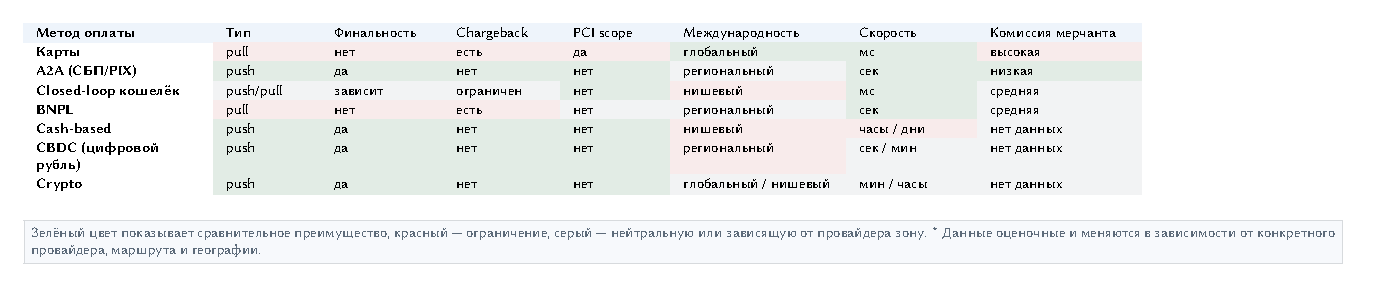
\includegraphics[width=\linewidth]{assets/figures/ch25-alternative-methods/alt-taxonomy-matrix.pdf}
  \caption{Матрица «Методы оплаты × параметры».}
  \label{fig:alt-taxonomy-matrix}
\end{figure}

Итак, таксономия нужна не ради красивой таблицы. Она помогает сравнивать
методы оплаты по платёжным контурам, финальности и распределению риска, а не по
маркетинговым обещаниям. С этой рамкой можно перейти к самому частому
источнику путаницы --- QR-платежам, за которыми стоят три разные модели.

\section{QR-платежи: три модели}
\label{sec:alt-qr}

QR-код --- это способ передать платёжную информацию без NFC-оборудования.
Сам по себе QR-код не является методом оплаты: за ним может стоять
карточная транзакция, A2A-перевод или замкнутый кошелёк. Различие между
моделями --- архитектурное, а не поверхностное.

Первая модель --- СБП, где QR выступает инициатором A2A-перевода. Динамический
QR в СБП --- это ссылка на платёжное поручение с реквизитами получателя,
суммой и purpose code. Клиент сканирует QR приложением своего банка; банк
формирует и направляет instant-перевод через инфраструктуру НСПК; мерчант
получает подтверждение за несколько секунд \sidecite{nspk-sbp}. Статический
QR содержит только реквизиты мерчанта без суммы, поэтому клиент вводит её
самостоятельно. Здесь нет chargeback, нет PCI scope, а комиссия обычно ниже
эквайринга.

Вторая модель --- Alipay и WeChat Pay. Здесь QR работает поверх
замкнутого кошелька (closed-loop wallet): пользователь либо сканирует QR
мерчанта, либо показывает мерчанту собственный QR из приложения. Платёж
происходит внутри экосистемы, а для внешнего мерчанта подключение обычно
идёт через локальных партнёров-эквайеров. В публичной документации
Alipay+ этот сценарий описан именно как merchant-presented mode, где QR
выпускает либо acquiring service provider, либо сама платформа, в
зависимости от entry code, order code и private order code
\sidecite{alipayplus-mpm}.

Третья модель --- PIX, бразильская система мгновенных платежей Banco Central
do Brasil, запущенная в 2020 году. Ключевое сходство с СБП --- мгновенный A2A-перевод,
финальность и низкие комиссии. Ключевое отличие --- PIX QR
(Pix Copia e Cola / QR Code Pix) стандартизирован так, что любой участник
системы принимает его без дополнительного двустороннего соглашения
\sidecite{pix}. Точные объёмы и сравнительные доли быстро меняются, поэтому
числовое сравнение с карточными транзакциями лучше вынести в онлайн-приложение.

\section{BNPL на уровне протокола}
\label{sec:alt-bnpl}

BNPL --- Buy Now Pay Later --- часто описывается как \enquote{современная
рассрочка}. На уровне протокола это удобно, но не совсем точно. При
стандартном BNPL-сценарии клиент на странице оплаты выбирает BNPL-провайдера
(Klarna, Affirm, Tabby, \enquote{Долями} и аналоги). Провайдер принимает
кредитное решение в реальном времени, мерчант получает полную сумму
немедленно, а клиент затем выплачивает её частями.

С точки зрения интеграции BNPL действительно похож на ещё одного эквайера:
обычно есть redirect или iframe, callback с результатом и webhooks для
статусов. Но экономически это другой контракт: кредитный риск живёт у
провайдера, а chargeback и спорные сценарии определяются договором,
а не схемными правилами Visa или Mastercard.

Регулирование BNPL быстро формируется и меняется. По состоянию на март
2026 года в России сервис рассрочки уже выделен в отдельный регулируемый
режим с реестром Банка России, а в ЕС BNPL включён в обновлённую
Consumer Credit Directive \sidecite{cbr-osr}\sidecite{eu-ccd-2023}. Для
печатной главы важнее зафиксировать именно этот институциональный сдвиг,
чем перечислять детали, которые устареют раньше тиража.

\begin{kaobox}[title=На практике]
  При выборе BNPL-провайдера стоит проверить три вещи: покрытие вашей
  аудитории, время кредитного решения под нагрузкой и модель ответственности
  за диспуты. Некоторые провайдеры не дают той же защиты, что карточные
  схемы, и это нужно понимать до интеграции.
\end{kaobox}

\section{Цифровой рубль: архитектура и сценарии}
\label{sec:alt-digital-ruble}

Цифровой рубль --- цифровая форма национальной валюты, эмитированная
Банком России непосредственно \sidecite{fz-340}\sidecite{cbr-digital-ruble}.
Это не безналичный рубль на счёте в коммерческом банке и не криптовалюта:
это третья форма денег наряду с наличными и безналичными, с отдельным
реестром обязательств на платформе Банка России.

Архитектура цифрового рубля трёхуровневая. Банк России выступает
эмитентом и оператором платформы, а коммерческие банки --- участниками,
которые открывают пользователям цифровые кошельки и обеспечивают вход
и выход средств. Клиент управляет кошельком через мобильное приложение
своего банка или Банка России \sidecite{cbr-digital-ruble}.

В чём отличие от безналичного рубля? В природе обязательства. Безналичный
рубль --- это обязательство коммерческого банка перед клиентом; цифровой
рубль --- прямое обязательство Банка России. Отсюда и вывод: для клиента
исчезает кредитный риск банка, а для банков возникает дискуссия о том,
как такая форма денег повлияет на депозитную базу \sidecite{cbr-digital-ruble}.

Отдельно обсуждаются условные платежи и смарт-контракты, а также
офлайн-режим. Для печатной главы разумно не изображать их как завершённый
массовый функционал: в текущих материалах Банка России офлайн назван
\enquote{возможностью в перспективе}, а смарт-контракты --- направлением
для инновационных сервисов \sidecite{cbr-digital-ruble}.

Где цифровой рубль пересекается с СБП? В том, что оба инструмента
инициированы государственным контуром и оба снижают стоимость платежа.
Но СБП --- это перевод безналичных рублей между счетами, а цифровой рубль
--- отдельная форма денег с отдельным кошельком. Смешивать их в одну
архитектуру нельзя \sidecite{cbr-digital-ruble}.

\section{Почему карточные контуры пока доминируют}
\label{sec:alt-card-dominance}

При наличии десятков альтернативных методов и активной поддержки A2A
во многих странах карты по-прежнему обрабатывают основную часть
потребительских транзакций. Почему?

Первая причина --- сетевые эффекты. Глобальные карточные схемы уже
обеспечили массовую эмиссию, приём и привычный пользовательский сценарий.
Мерчант, который принимает карты, автоматически охватывает почти всех
покупателей. Новый метод должен одновременно получить поддержку
со стороны эквайера и эмитента, а это самый трудный вариант сетевого
эффекта.

Вторая причина --- международность. Карта, выпущенная в одной стране,
работает в десятках и сотнях других по единому протоколу. Локальные
A2A-системы --- СБП, PIX, UPI --- обычно не взаимозаменяемы.

Третья причина --- защита покупателя. Chargeback --- это механизм, который
A2A-системы не воспроизводят без изменения самой идеи финальности.
Покупатель, оплативший картой незнакомому мерчанту, имеет формальный
возвратный контур; покупатель, оплативший через A2A, чаще остаётся с
договорной защитой, а не с схемным chargeback.

Наконец, четвёртая причина --- инфраструктурная инерция. Десятки миллионов
POS-терминалов уже сертифицированы для карточных схем. Переоснащение
или добавление нового метода окупается только при массовом спросе, а
массовый спрос не возникает, пока мерчанты не видят достаточного
пользовательского потока. Это классический замкнутый круг внедрения.

Альтернативные методы выигрывают в нишах: низкая комиссия для A2A,
доступность для небанковских клиентов в cash-based, условные платежи в
CBDC, рассрочка в BNPL. Но глобальную универсальность и инфраструктурный
охват карт они пока не воспроизводят.

\section{Payment method mix для РФ и СНГ}
\label{sec:alt-mix}

Подробные доли по странам и годам быстро устаревают, поэтому для печатной
главы полезнее держать паттерны, а не цифры.

Россия --- это сочетание массового карточного приёма, быстро растущего
A2A-контура в виде СБП и сильной роли локальных требований. Казахстан заметно
сильнее завязан на экосистемные сценарии и QR вокруг Kaspi. Узбекистан
живёт с выраженной ролью локальных карточных схем HUMO и UzCard, а
международные карты сильнее проявляются в трансграничных сценариях.
Армения и ряд других стран СНГ демонстрируют смешанный ландшафт: локальная
схема для внутренних платежей и Visa/Mastercard для международного приёма.

Этого достаточно для продуктового вывода: СНГ не является единым платёжным
рынком. При локализации нельзя копировать российскую структуру способов оплаты на
Казахстан или армянский сценарий на Узбекистан без проверки локального
оператора платёжного контура, доли QR и регуляторных требований.

\begin{kaobox}[title=На практике]
  При локализации платёжного сценария в новой стране СНГ рекомендуется
  провести три проверки: доля локальных карт против международных в BIN-
  распределении вашего трафика (влияет на interchange и долю успешного приёма),
  наличие локального A2A-метода с массовым принятием и законодательные
  требования к обязательному приёму локальных карт.
\end{kaobox}

\begin{chaptersummary}
\begin{itemize}
  \item Шесть классов методов оплаты --- карты, A2A, кошельки, BNPL,
        cash-based и CBDC/crypto --- различаются по типу (push/pull),
        финальности, chargeback, PCI scope и международному охвату.
  \item QR --- это способ запустить нужный контур, а не отдельный метод оплаты:
        СБП QR ведёт в A2A, Alipay QR --- в closed-loop wallet, PIX QR ---
        в мгновенный A2A-перевод.
  \item BNPL на уровне протокола --- это кредитное решение в реальном
        времени, немедленная выплата мерчанту и рассрочка для клиента;
        риски и споры определяются договором с провайдером.
  \item Цифровой рубль --- третья форма денег: кошелёк живёт на платформе
        Банка России, а не в коммерческом банке; смарт-контракты и офлайн-
        режим следует проверять по текущим материалам регулятора.
  \item Карточные контуры доминируют благодаря сетевым эффектам,
        международности, защите покупателя и инфраструктурной инерции;
        альтернативы выигрывают в нишах.
  \item Структуру способов оплаты по РФ и СНГ лучше читать как карту паттернов,
        а не как вечную таблицу процентов: локальный контекст здесь важнее
        усреднённого глобального вывода.
\end{itemize}
\end{chaptersummary}
